\chapter{Theoretical Literature}

\section{User experience}
According to International Organization for Standardization the official definition of user experience is: 
\begin{displayquote}
    \textit{A user's perception and responses resulting from the use and/or anticipated use of a product, system or service.
    User's perceptions and responses include the user's emotions, beliefs, preferences, perceptions, comfort, behaviours and accomplishments that occur before, during and after use.}

    (\href{https://www.iso.org/obp/ui/#iso:std:iso:9241:-210:ed-2:v1:en}{ISO 9241-11:2019, subsection 3.15}).
\end{displayquote}

Briefly said, user experience, UX for short, is about \textbf{not} placing yourself, but \textbf{the users} in the center of the design process. \underline{Their} journey should be easy and straight forward as possible. The goal is understand the user's motivations behaviours, needs and concerns. Although user experience sounds like something you don't know very well your constantly surrounded by both good and bad user experiences. Below are 2 examples.

\subsection{The Norman door}
The Norman door is named after Don Norman. Don Norman is the author of "The Design of Everyday Things" \cite{Norman2013}. He is considered one of the patriarchs of user experience. A door is considered a Norman door when the design tells you to do the opposite of what you are actually supposed to do or gives the wrong signal and needs a sign to correct it.
A possible solution is a door with no handles. If there are no handles, you can only \underline{push}, to open the door.

\subsection{Tomato ketchup}
Around 1889 Heinz introduced its octagonal glass ketchup bottle. The iconic glass bottle was their staple for over a hundred years. But in the world of user experience research not the glass bottle, but the current plastic bottle is known as one of the greatest innovations since the invention of semiconductors. (\textit{slightly exaggerated})

\subsubsection{Innovations}
Although Heinz had no intention to reinvent their ketchup bottle, it was determined to better understand how people were consuming its ketchup at home. 
The company did an extensive market-research in which researcher visited ordinary families and watched the way they used their ketchup. Something remarkable happened. Something that \textit{probably} exceeded their greatest expectations.

Casey Keller, who was the chief growth offer for Heinz at the time, said: 

\begin{displayquote}
    \textit{
    "I remember sitting in one of those households, There was a three-year-old and a six-year-old, and what happened was that the kids asked for ketchup and Mom brought it out. It was a forty-ounce bottle. And the three-year-old went to grab it himself, and Mom intercepted the bottle and said, 'No you are not going to do that.' She physically took the bottle away and doled out a little dollop. You could see that the whole thing was a bummer."}
\end{displayquote}

Researchers had already discovered that children consume approximately 60\% \textbf{ more} ketchup than an adult. But now, they found out that their biggest consumers, children, did not have direct access to the bottle and for as long as the parents are in control they would always restrain the consumption levels. 

The result was a so called, \textit{EZ Squirt bottle}. A bottle completely made out of plastic with a cone-shaped tip. After thoroughly analyzing the families that used this new bottle, it turned out to be a \underline{great success}. The new ketchup bottle led to a consumption growth of \textbf{12\%}!

Heinz did not stop there, it continued reinventing its bottle. In the beginning of the 21st century, after the sales were down, Heinz decided to conduct another user research. The researchers concluded that consumers struggled to get the leftovers out of the bottle. Instead of buying a new bottle, they would keep using the leftover ketchup they could squeeze out, often this was less than they wanted. Getting the leftovers out was unpleasant and often messy task. To fight this, people often stored their bottle upside down in the refrigerator. 

Again, Heinz came up with a great solution. They decided to turn the bottle over. And so, \texit{the current} Heinz upside-down ketchup bottle was born.
You can find the result in \autoref{fig:heinz-ketchup-bottle}

\begin{figure}[h!]
\centering
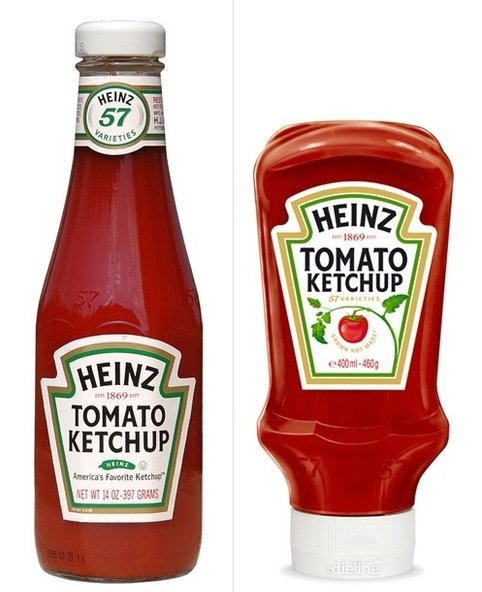
\includegraphics[scale=0.2]{figures/ketchup.png}
\caption{Heinz's tomato ketchup bottle before and after the innovation.}
\label{fig:heinz-ketchup-bottle}
\end{figure}

\section{Personas}
    A persona is a fictional character that represent the \underline{ideal target} you should design for and communicate with. They help us make the best decisions and address their specific problems and pain points. There are 2 types of personas: Buyer personas and User personas. 
    
    \subsection{Buyer personas}
    Buyer personas represent those who \underline{buy} the product or service or those that can encouraged buying as outcome. Although buyer personas are often an added value, they will not be expressly used in this paper.
    
    \subsection{User personas}
    User personas represent those who \underline{use} the product or service. A user persona may or may not be the one that has the authority to buy the product or service. Regardless, they often greatly affect the buying process. There can be an overlap between both persona types.
    
    User personas are usually divided into \underline{four} categories. Only the first \underline{three} are \textit{considerably} related to this paper.

    \begin{itemize}
        \item{Goal-directed persona}
        \item{Role-based persona}
        \item{Engaging persona}
        \item{\textit{Fictional persona}}
    \end{itemize}
    
    \subsubsection{The goal-directed persona}
        This perspective focuses on what the typical user wants \underline{to do} with the product. As a \gls{ux} researcher you want to examine the process a user would prefer to utilise in order to achieve their objectives. The goal-directed perspective is beautifully displayed in \autoref{fig:goal-directed-persona-perspective}. 
        
       \begin{center} 
        \textit{Author/Copyright holder: Smashing Magazine.}
       \end{center} 
       
        \begin{figure}[h]
            \centering
            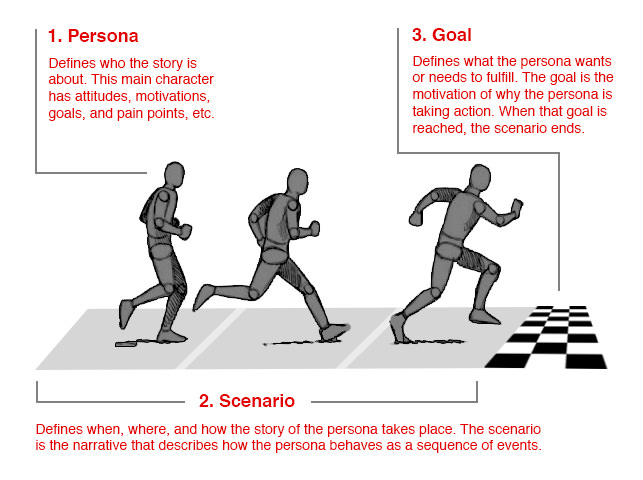
\includegraphics[scale=0.5]{goal-directed-perspective.jpg}
            \caption{Goal-directed persona perspective}
            \label{fig:goal-directed-persona-perspective}
        \end{figure}
    \subsubsection{The role-based persona}
    The role-based perspective is also a goal-directed perspective, but they are mainly focused on the role of the user inside the organization. A role-based persona should give an answer to the following questions.
    \begin{itemize}
        \item{Where will users use our product?}
        \item{What is the purpose of the product?}
        \item{What business objectives are required and what can be achieved with them?}
        \item{Which people will be impacted by its role?}
        \item{What kind of functions are being served?}
    \end{itemize}
    
    \subsubsection{The engaging persona}
    
    The engaging personas are distinguished by their very realistic persona descriptions. The other persona types tend to be too stereotypical. The designers are not able to envision their lives. These personas are therefore specifically designed so that the designers who use them can become more engaged with them.
    
    \section{User stories}
    A key component of agile development is putting people \textbf{first}. A user story is a description of an end goal from a user's perspective. It's purpose is to articulate how a piece of work will return great value back to the customer. Note that "customers" don't have to be the end users. This can also be a colleague who depends on your team.
    
    Important to understand is that user stories are \underline{not} a way to write requirements. The User Stories help us start the right conversation about the users' needs, but don't go into detail. Eventually requirements are added once they are agreed upon by the team.
    
    \subsection{User story templates}
        User stories are often created based on a template. The most common template is the \textbf{Connextra} template or the three-part user story template. It highlights the who, the what and the why from the user's perspective. This template will also be used further down the paper.
        
    \begin{minted}{javascript}
        As a <role> I can <capability>, so that <receive benefit>.
    \end{minted}
    
    \begin{itemize}
        \item{\mintinline{javascript}{As a <role>} is often misinterpreted. A role is not a profession or job title, but a user persona. It is therefore important that the team has a shared understanding of this user persona. They should understand what he is working on, what he thinks and what he feels.}
        \item{\mintinline{javascript}{I can <capability>} describes the intent, \underline{not the features} they use. What are the users trying to achieve? If you're describing any part of the \gls{ui} and not what the user's goal is you are incorrect.}
        \item{\mintinline{javascript}{so that <receive benefit>} describes the user's end goal. this clause is seen as optional but often very helpful. In complex environment it will improve the general description of the user story.}
    \end{itemize}  
         
    The creator of the Connextra template, \href{https://en.wikipedia.org/wiki/Mike_Cohn/}{Mike Cohn}, recently wrote an article about why you should use the three-part template. Here is \href{https://www.mountaingoatsoftware.com/blog/why-the-three-part-user-story-template-works-so-well}{\underline{link}} to the article.
    
   \section{User flow}
    A user flow is a series of actions a prototypical user takes to accomplish a certain goal. 
    Projects often have many stakeholders, requirements and limitations causing the user not being the central role in the design. By making user stories, we don't only ensure that the user remains the point of focus but it is a great tool for developers to show how the product or service should work.
    
    \section{Prototyping}
    A prototype is rudimentary working sample of a product or service built to test if a certain concept or process works. It is a \textbf{low cost} way to reduce the risk that the idea may not perform as intended, \textit{however generally it cannot eliminate all risk}. Prototyping helps you assure that only \textit{the best version} of something goes forward.
    
    Prototyping has several important benefits: 
    \begin{itemize}
        \item {You receive valuable feedback from the users early the process.}
        \item { Compared to development, prototyping is a very efficient and effective process, especially when several rounds are required to fine-tune the outcome. }
        \item {Prototypes are a great way to check if the customer's requirements correspond to the design. }
        \item {Completed prototypes allow the software engineers insight into the accuracy of initial project estimates and whether the proposed deadlines and milestones can be met.}
        
    \end{itemize}
    
    
    \section{Usability testing} 
    Usability testing involves watching representative users working with your product or service so that you can make improvements based on their actions. Usability testing gives you invaluable feedback on how users behave with your product or service. Knowing how your users behave helps you create a much suitable product or service. 
    Rather than guessing about what your users might like or need, you can see their usage first handed. 
    
    \subsection{Moderated usability testing}  
    Moderated usability testing is when the user completes a set of tasks, \textbf{whilst being observed by a moderator (researcher).} Moderated usability has many benefits: 
    
    \begin{itemize}
        \item { You receive immediate feedback, so that important details are not lost.}
        \item { You can answer any immediate questions posed by the user.}
        \item { You have the ability to guide users through tasks.}
        \item { Early prototyping may contain unfinished features which can cause confusion. By being physically present you can clarify on the spot.}
        \item { You have an overview on all tasks the user performs, both active and passive.}
    \end{itemize} 
    
    However, moderated usability testing has a \textit{major} drawback. Moderated user tests are greatly affected by \textbf{the Hawthorne effect}.

    \subsubsection{The Hawthorne effect}
    The Hawthorne effect occurs when people behave differently because they know that they are being observed. The term was first introduced by H. A. Landsberger who was conducting research at the \underline{Hawthorne Works factory}. The factory wanted to investigate whether the employees would become more productive with higher light intensities. 
    
    At first the productivity seemed to have increased considerably, but it completely plunged after the experiment ended. The production gain was due to the motivational effect. The workers performed better because of the interest that was being shown in them.